\documentclass[UTF8]{ctexart}
\usepackage{graphicx}
\usepackage{amsmath}

\title{Paper Reading Note \\ Deep Learning for Chinese Word Segmentation and POS Tagging}
\author{BrightHush}
\date{\today}

\begin{document}
\maketitle
\tableofcontents

\newcommand{\figref}[1]{\figurename~\ref{#1}}

\section{Abstract}
这篇文章的主要思路是使用DNN训练得到的字向量作为Word Segmentation或者POS Tagging的输入特征。对于每一句话作为一个sample,对
sentence中的每个词,取窗口大小为$w$,将窗口中的字对应的向量连接成为输入特征。对sentence进行标记使用的训练方法是三层神经网络加上
Viterbi算法,神经网络的输出层为当前窗口的中心词对应为每个tag的可能性(得分),Viterbi算法则是根据句中每个词对应tag的可能行(得分),求解一个最大的可能(得分)的tag序列作为输出。对于如何对该模型进行训练,文中提到了两种方法,一种是Sentence-Level Log-Likelihood方法,另外一种是Perceptron Algorithm。

\section{Model}

\begin{figure}
\centering
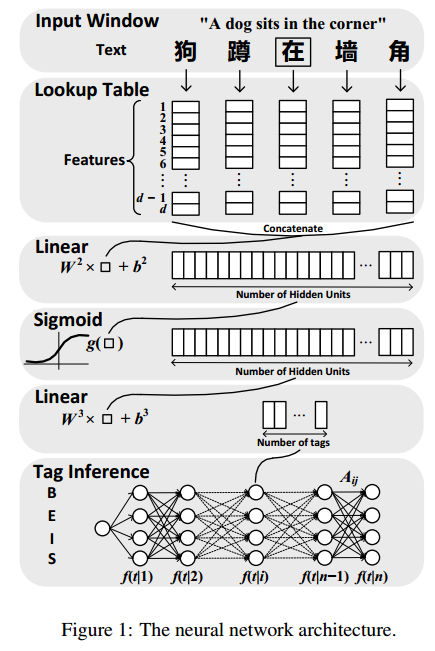
\includegraphics[width=0.8\textwidth]{NeuralNetworkArchitecture}
\caption{Neural Network Architecture}
\label{Figure One}
\end{figure}

该模型的整体架构图可以参见 \figref{Figure One}。

\subsection{Character to Vector}
对于字对应到向量我们可以认为是通过查表操作得到,字典用$D$表示,字向量存储在character embedding matrix $M \in R^{d \cdot |D|}$,
其中$d$ is the dimensionality of the vector, and $|D|$ is the size of the dictionary.
\\
For a Chinese sentence $c_{[1:n]}$ consist of $n$ characters $c_i$, $1 \geq i \geq n$. 对于字$c_i \in D$对应在embedding 
matrix中的列号为$k_i$,查表操作可以表示为$Z_D(C_i)=Me_{k_i}$,其中$e_{k_i} \in R^{|D| \cdot 1}$,是一个列向量,只有行$k_i$为1,其余行为0.

\subsection{Tag scoring}
神经网络第$l$层的变换可以视为函数$f_{\theta}^{l}(\cdot)$,那么$L$层的神经网络可以表示成为:
\begin{equation}
f_{\theta}(\cdot)=f_{\theta}^L(f_{\theta}^{L-1}(...f_{\theta}^1(\cdot)...))
\end{equation}
对于句子$c_{[1:n]}$,我们取窗口大小为$w$,那么在位置$i$的词$c_i$对应的输入特征向量可以表示为:
\begin{equation}
f_{\theta}^1(c_i)=\begin{pmatrix}
Z_D (c_{i-w/2}) \\ . \\ . \\ . \\ Z_D(c_i) \\ . \\ . \\ . \\Z_D(c_{i+w/2})
\end{pmatrix}
\end{equation}
其中每个字对应的$Z_D(c_i)$都是列向量。\\
神经网络的输出为字$c_i$为某一个tag的score,因此输出层的神经元个数为$|\tau|$(表示使用到的tag总数),那么\figref{Figure One}中的
神经网络可以表示为下面的公式:
\begin{equation}
f_{\theta}(c_i)=f_{\theta}^3(g(f_{\theta}^2(f_{\theta}^1(c_i)))) \\
=W^3g(W^2f_{\theta}^1(c_i)+b^2)+b^3
\end{equation}
其中$W^2 \in R^{H \times (wd)}$,$b^2 \in R^H$,$W^3 \in R^{|\tau| \times H}$,并且$b^3 \in R^{|\tau|}$,$H$表示隐藏
层的神经元个数,非线性函数选择sigmoid函数$g(x)=1/(1+e^{-x})$。

\subsection{Tag Inference}
由于字对应的tag之间存在比较大的依赖关系,那么我们定义transition score $A_{ij}$表示连着的字符从标记$i \in \tau$转移到标记
$j \in \tau$的得分。那么对于一个句子$c_{[1:n]}$,神经网络得到的是评分矩阵$f_{\theta}(c_{[1:n]})$,我们使用$f_{\theta}(t|i)$
表示在神经网络参数为$\theta$的情况下,句子第$i$个字被标记为$t$的得分。那么一个句子$c_{[1:n]}$对应标记序列为$t_{[1:n]}$的得分可以计
算为:
\begin{equation}
s(c_{[1:n]}, t_{[1:n]}, \theta) = \sum_{i=1}^n(A_{t_{i-1}t_i} + f_{\theta}(t_i|i))
\label{setence score}
\end{equation}
对于一个给定的句子,我们可以通过Viterbi算法求的得分最大的标记序列$t_{[1:n]}^*$。


\section{Training Algorithm}
根据模型建立的情况,我们可以得到参数$\theta = (M, W^2, b^2, W^3, b^3, A)$,我们需要从训练数据中训练得到参数$\theta$是的似然函数
最大,这个似然函数当然是建立在训练集$R$上面的:
\begin{equation}
\theta -> \sum_{\forall (c,t) \in R} logp(t|c, \theta)
\label{log-likelihood}
\end{equation}
对于需要最大化log似然\ref{log-likelihood},可以使用梯度上升法(gradient ascent algorithm),对于每一个样本$(c,t)$我们可以使用下面的
方法更新梯度:
\begin{equation}
\theta <- \theta + \lambda \frac{\partial logp(t|c,\theta)}{\partial \theta}
\label{gradient ascent update}
\end{equation}
当然对于神经网络中的参数求导,可以根据求导的链式法则直到character embedding layer。

\subsection{Sentence-Level Log-Likelihood}
对于按照\ref{setence score}我们可以得到句子对应标记序列的得分,那么我们可以构造指数函数来表示句子对应该标记序列的概率,于是对于所有的样本
句子我们便可以得到样本集的似然。
\begin{equation}
p(t|c, \theta) = \frac{e^{s(c, t, \theta)}}{\sum_{\forall (t^{\textquoteleft})}e^{s(c, t^{\textquoteleft}, \theta)}}
\label{setence probability}
\end{equation}
那么句子标记概率的log可以表示为下面的公式:
\begin{equation}
logp(t|c, \theta) = s(c, t, \theta) - log \sum_{\forall t^{\textquoteleft}} e^{s(c, t^{\textquoteleft}, \theta)}
\end{equation}
\\
从条件概率的计算公式中,我们可以看到要计算所有路径的得分情况,这个路径的数量是随着句子长度指数级增长的,所以计算非常耗时。所以论文中引用了另外
一种比较快捷的计算方式,也就是下面将提到的方法。

\subsection{Perceptron Algorithm}
这里将提到的方法是收到Collins, 2002相关工作的启发,对于每一个给定的样本(c,t),神经网络得到句中各个字对应的得分情况记为$f_{\theta}(c)$,
那么根据$f_{\theta}(c)$和$A$使用Viterbi算法可以得到得分最高的标记序列$t^{\textquoteleft}$,那么对于句中的每个字$c_i$,
如果$t_i \neq t_{i^{\textquoteleft}}$:
\begin{equation}
\frac{\partial L_{\theta} (t, t^{\textquoteleft} | c)}{\partial f_{\theta}(t_i|i)}++, 
\frac{\partial L_{\theta} (t, t^{\textquoteleft} | c)}{\partial f_{\theta}(t_{i^{\textquoteleft}}|i)}--
\end{equation}

对于$c_i$对应的转移情况,如果存在$t_{i-1} \neq t_{i-1}^{\textquoteleft}$或者$t_i \neq t_{i}^{\textquoteleft}$:
\begin{equation}
\frac{\partial L_{\theta} (t, t^{\textquoteleft} | c)}{\partial A_{t_{i-1}t_i}}++, 
\frac{\partial L_{\theta} (t, t^{\textquoteleft} | c)}{\partial A_{t_{i-1}^{\textquoteleft}t_{i}^{\textquoteleft}}}--
\end{equation}
感官上这种做法有点像是对正确预测的tag sequence进行奖励,对错误预测tag sequence进行惩罚。之前该Perceptron Algorithm是用来计算
HMM-style tagger,这里我们用来计算参数更新的方向。

\section{References}
\begin{description}
\item[][1] Xiaoqing Zheng, Hanyang Chen, Tianyu Xu, Deep Learning for Chinese Word Segmentation and POS Tagging,
Proceedings of the 2013 Conference on Empirical Methods in Natural Language Processing, pages 647-657.

\end{description}

\end{document}
